\documentclass{article}
\usepackage[margin=1in]{geometry}
\usepackage{amsmath}
\usepackage{amssymb}
\usepackage{mathtools}
\usepackage{float}
\usepackage{tikz}
\usetikzlibrary{automata, positioning, arrows}
\tikzset{
    ->,
    >=stealth',
    node distance=3cm,
    every state/.style={thick, fill=gray!10}, 
    initial text=$ $, 
}
\title{Title}
\author{Ty Butler}

\newcommand{\thm}[1]{\textbf{Theorem #1}}
\newcommand{\Nat}{\mathbb{N}}
\newcommand{\Int}{\mathbb{Z}}
\newcommand{\Rat}{\mathbb{Q}}
\newcommand{\Real}{\mathbb{R}}
\newcommand{\Comp}{\mathbb{C}}

\begin{document}
\maketitle{}

\section{}
\subsection{}
Suppose there existed no path of width at least $\frac{F}{m}$. Since there are $m$ edges in the graph, there are at most $m$ paths from $s$ to $t$. Since each path has less than $\frac{F}{m}$ capacity, the total capacity of all paths is less than $\frac{F}{m} m = F$. Consider a cut separating $s$ from $t$. Since the maximum capacity of all paths is less than $F$, the capacity of the cut must necessarily be less than $F$, as it encompasses all paths. Since such a cut exists, any minimum cut will also have a capacity less than $F$. Therefore, by the max-flow min-cut theorem, the max flow from $s$ to $t$ is less than $F$. This is a contradiction, as $F$ cannot be less than $F$, and therefore our assumption that no path of width at least $\frac{F}{m}$ exists must be false. 

\subsection{}
As a result of $a$, the widest path must have a width of at least $\frac{F}{m}$. Pushing flow on this path once will reduce the total capacity of the residual graph by at least $\frac{F}{m}$. After $k$ applications of the process, the capacity on the residual graph will be $K - k\frac{F}{m}$, where $K$ is the initial total capacity. Therefore the residual graph will have capacity $0$ in at most as many steps as it takes for $K = k\frac{F}{m}$, or $k = \frac{m}{F}K$. As a fraction, this is $\frac{K - k\frac{F}{m}}{K}$, or $1 - \frac{k\frac{F}{m}}{K}$, or, at most $e^{\frac{Fk}{mK}}$, equivalently, 

\end{document}

\iffalse
example fsm
\begin{figure}
    \centering
    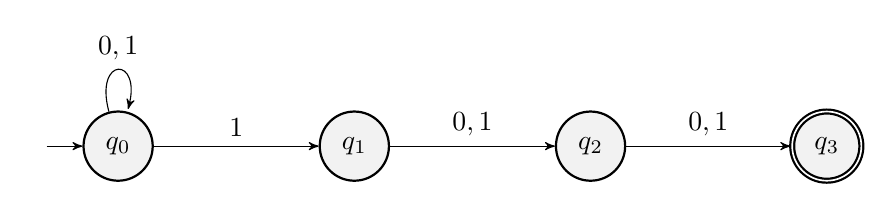
\begin{tikzpicture}
        \node[state, initial] (q0) {$q_0$};
        \node[state, right of=q0] (q1) {$q_1$};
        \node[state, right of=q1] (q2) {$q_2$};
        \node[state, accepting, right of=q2] (q3) {$q_3$};

        \draw 
            (q0) edge[loop above] node{$0,1$} (q0)
            (q0) edge[above] node{$1$} (q1)
            (q1) edge[above] node{$0,1$} (q2)
            (q2) edge[above] node{$0,1$} (q3);
    \end{tikzpicture}
\end{figure}
\fi
